\chapter{Results}
This chapter presents all the results for the algorithms and computations mentioned in the previous chapters. As a brief reminder, the \emph{paraphrased} setting operates with samples from the datasets $\si \in D$ and $\spi \in D_p$ (see Equation~\ref{eq:paraphrasing}) while the \emph{model-generated} setting operates with samples from the dataset $\si \in D$ and $\smi \in D_m$ (see Equation~\ref{eq:model_generated_sample}. Concretely, the evaluation checks whether flattened gradients $\vXspi[\theta]$ (paraphrased) and $\vXsmi[\theta]$ (model-generated) retrieve their corresponding original samples $\vXsi[\theta]$ via cosine similarity, following Equation~\ref{eq:cosine_similarity_paraphrased} and the accuracy metric defined in Equation~\ref{eq:accuracy_bm25}.
\\\\
The remainder of the chapter is organized as follows. Section~\ref{sec:baseline_perf} reports baseline retrieval results using the full model gradient. Section~\ref{sec:single_layer_perf} analyzes contributions per component. Section~\ref{sec:layer_vs_full} compares single-component scores to full-model scores. Section~\ref{sec:greedy_vs_rp} evaluates compact surrogates via forward greedy selection against a random-projection baseline. Section~\ref{sec:exec_time} summarizes the cost profile.

\section{Performance of Gradient Similarity as an Explanation Method}\label{sec:baseline_perf}
All gradient similarities are computed and reconstructed from stored dot products using Equations~\ref{eq:dot_grad_decompose} to represent the cosine similarities for both the paraphrased ($\simcos(\vXspi, \vXsj)$) and the model-generated ($\simcos(\vXsmi, \vXsj)$) case, $\forall \spi \in D_p$ and $\forall \smi \in D_m$. To avoid the comparison of all-pairs $\mathcal{O}(N^2)$, for each paraphrased (or model-generated) sample $\sj \in \mathcal{C}_i(b)$ is restricted to a BM25 candidate set with $b=5$ (Algorithm~\ref{alg:bm25_select_samples}). The metrics $\operatorname{accuracy}^{(b)}_{\theta}(D_p,D)$ and $\operatorname{accuracy}^{(b)}_{\theta}(D_m,D)$ are then evaluated as in Equation~\ref{eq:accuracy_bm25}.
\begin{table}[htb]
    \centering
    \begin{tabular}{|l|c|c|}
        \hline
        \textbf{Model} & \textbf{Paraphrased} & \textbf{Model-generated} \\
        \hline
        AMD-OLMo-1B-SFT & 0.993 & 0.218 \\
        \hline
    \end{tabular}
    \caption{Score for $\operatorname{accuracy}^{(b)}_{\theta}(D_p,D)$ (paraphrased) and $\operatorname{accuracy}^{(b)}_{\theta}(D_m,D)$ (model-generated) cases with the full model gradient.}
    \label{tab:model_accuracy}
\end{table}
As shown in Table~\ref{tab:model_accuracy}, the gradient similarity method is able to find nearly all original samples when queried with the paraphrased samples of $D_p$. For the model-generated setting, this is very different, as it can only identify approximately one out of five original samples when queried with the dataset $D_m$. When considering that random guessing would lead to a baseline of $0.2$ due to the candidate set having a size of $\lvert\mathcal{C}_i(b)\rvert = 5$ since $b=5$ and $1 \div 5=0.2$, the accuracy is not far off.
\\\\
In the paraphrased setting, only seven samples are wrongly assigned to their original counterparts. It seems that they are not wrongly assigned by coincidence, they are connected by some patterns. For example, three of them (with the ids lima\_725, lima\_767 and lima\_773) have very long assistant messages resulting in token sequences with more than $2950$ items, despite \texttt{AMD-OLMo-1B-SFT} only having a context size of $2048$. 
\fxnote{Illustrate similarites between samples that have been classified wrongly and give a short example}

\section{Single Layer Performance}\label{sec:single_layer_perf}
This section quantifies the contribution of \emph{single} layer components to retrieval and similarity. For each parameter matrix $\Wlk$, the BM25-restricted retrieval accuracy $\operatorname{accuracy}^{(b)}_{\Wlk}(\cdot,D)$ (Equation~\ref{eq:layer_accuracy_bm25}) is evaluated to test whether the gradient of a \emph{single} component suffices to recover the original sample. All quantities are reconstructed from per-component dot products (Section~\ref{subsec:intermediate_results}), so no full gradients are materialized.
\\\\
The results are reported for both settings (\textbf{paraphrased} and \textbf{model-generated}), aggregated across depth and component family (Embedding; Attention $Q/K/V/O$; MLP gate/up/down). The medians across layers are shown for robustness against outliers (Table~\ref{tab:average_accuracy_layer_component}), and depth-wise trends are visualized in Figures~\ref{fig:paraphrased_accuracy_per_layer}~and~\ref{fig:model_generated_accuracy_per_layer}.
\begin{table}[h]
    \centering
    \begin{tabular}{|c|c|c|c|}
        \hline
        & \textbf{Layer Component} & \textbf{Paraphrased} & \textbf{Model-generated} \\
        \hline
        \multirow{1}{5em}{Embedding}
        & Embedding & 0.993 & 0.231 \\
        \hline
        \multirow{4}{5em}{Attention}
        & Query-Projection & 0.979 & 0.253 \\
        & Key-Projection & 0.916 & 0.211 \\
        & Value-Projection & 0.982 & 0.188 \\
        & Output-Projection & 0.994 & 0.205 \\
        \hline
        \multirow{3}{5em}{MLP}
        & Gate-Projection & 0.994 & 0.265 \\
        & Up-Projection & 0.993 & 0.26 \\
        & Down-Projection & 0.995 & 0.221 \\
        \hline
    \end{tabular}
    \caption{Averaged (median) layer component accuracy for the paraphrased ($\operatorname{accuracy}^{(b)}_{\Wlk}(D_p,D)$) and the model-generated ($\operatorname{accuracy}^{(b)}_{\Wlk}(D_m,D)$) case. \fxnote{also include mean}}
    \label{tab:average_accuracy_layer_component}
\end{table}
As shown in Table\ref{tab:average_accuracy_layer_component}, single-component gradients already suffice to recover the original item in the \emph{paraphrased} setting: median accuracies exceed $0.98$ for all components except the key projection ($0.916$), with the MLP path (gate/up/down) and the attention output projection matching or slightly surpassing the full-model score ($\approx 0.99$). This indicates that paraphrasing preserves gradient directions consistently across layers, so gradients from individual components contain enough information to identify the correct original sample. In contrast, the \emph{model-generated} setting collapses toward the $0.2$ chance level imposed by $b{=}5$: accuracies cluster near baseline, with only the MLP (gate/up at $\approx 0.26$) and the query projection ($0.253$) providing a small, repeatable improvement; the value projection falls below chance ($0.188$). The embedding matrix reaches $0.231$, suggesting that lexical overlap alone is insufficient once responses are re-synthesized. Overall, the information that supports correct retrieval is broadly distributed in the paraphrased condition but becomes concentrated mainly in the MLP and $Q$ projections in the model-generated condition, while $K$ and $V$ contribute the least to this retrieval objective.

\subsection{Does Size matter?}
Here, \emph{size} refers to the number of parameters in a component ($4{,}194{,}304$ for the attention projections $Q/K/V/O$,
$16{,}777{,}216$ for the MLP projections gate/up/down, and $103{,}022{,}592$ for the embedding).  Figure~\ref{fig:accuracy_per_layer_boxplot} summarizes top-1 retrieval accuracy for these three bins; the subpanels
(Figs.~\ref{fig:accuracy_per_layer_boxplot_paraphrased}–\ref{fig:accuracy_per_layer_boxplot_model_generated}) correspond to the \emph{paraphrased} and \emph{model-generated} settings, respectively.
\\\\
In the \emph{paraphrased} condition (Fig.~\ref{fig:accuracy_per_layer_boxplot_paraphrased}), accuracies are essentially at ceiling across all sizes. The $4{,}194{,}304$ group exhibits a wider spread with several low outliers, whereas the $16{,}777{,}216$ group is tightly clustered near $0.99$ and the $103{,}022{,}592$ point (embedding) is likewise close to $0.99$. These differences are small. Because cosine similarity normalizes vector magnitudes, the slight improvement observed for larger components is best interpreted as reduced variance rather than a substantive size effect.
\\\\
In the \emph{model-generated} condition
(Fig.~\ref{fig:accuracy_per_layer_boxplot_model_generated}), all groups concentrate around the $0.2$ chance level imposed by $b{=}5$. The $16{,}777{,}216$ group attains a marginally higher median ($\approx 0.24$–$0.25$) than the $4{,}194{,}304$ group
($\approx 0.21$–$0.23$), and the embedding ($103{,}022{,}592$) sits at $\approx 0.23$. Dispersion is largest for the $4{,}194{,}304$ group, which bundles both relatively stronger (e.g., $Q$) and weaker (e.g., $V$) projections despite identical size. This pattern indicates that \emph{component type}, not parameter count, drives the modest differences: MLP projections outperform on average, whereas $K$/$V$ lag, even though all four attention projections share the same size.
\\\\
Overall, there is no meaningful monotonic relationship between parameter count and retrieval accuracy. In the paraphrased setting, performance is uniformly high regardless of size; in the model-generated setting, accuracy
hovers near chance with only slight advantages for MLP-sized components. The functional role of a component within the architecture matters more than how many parameters it contains.
\begin{figure}[h]
    \centering
    \begin{subfigure}[h]{0.495\textwidth}
        \centering
        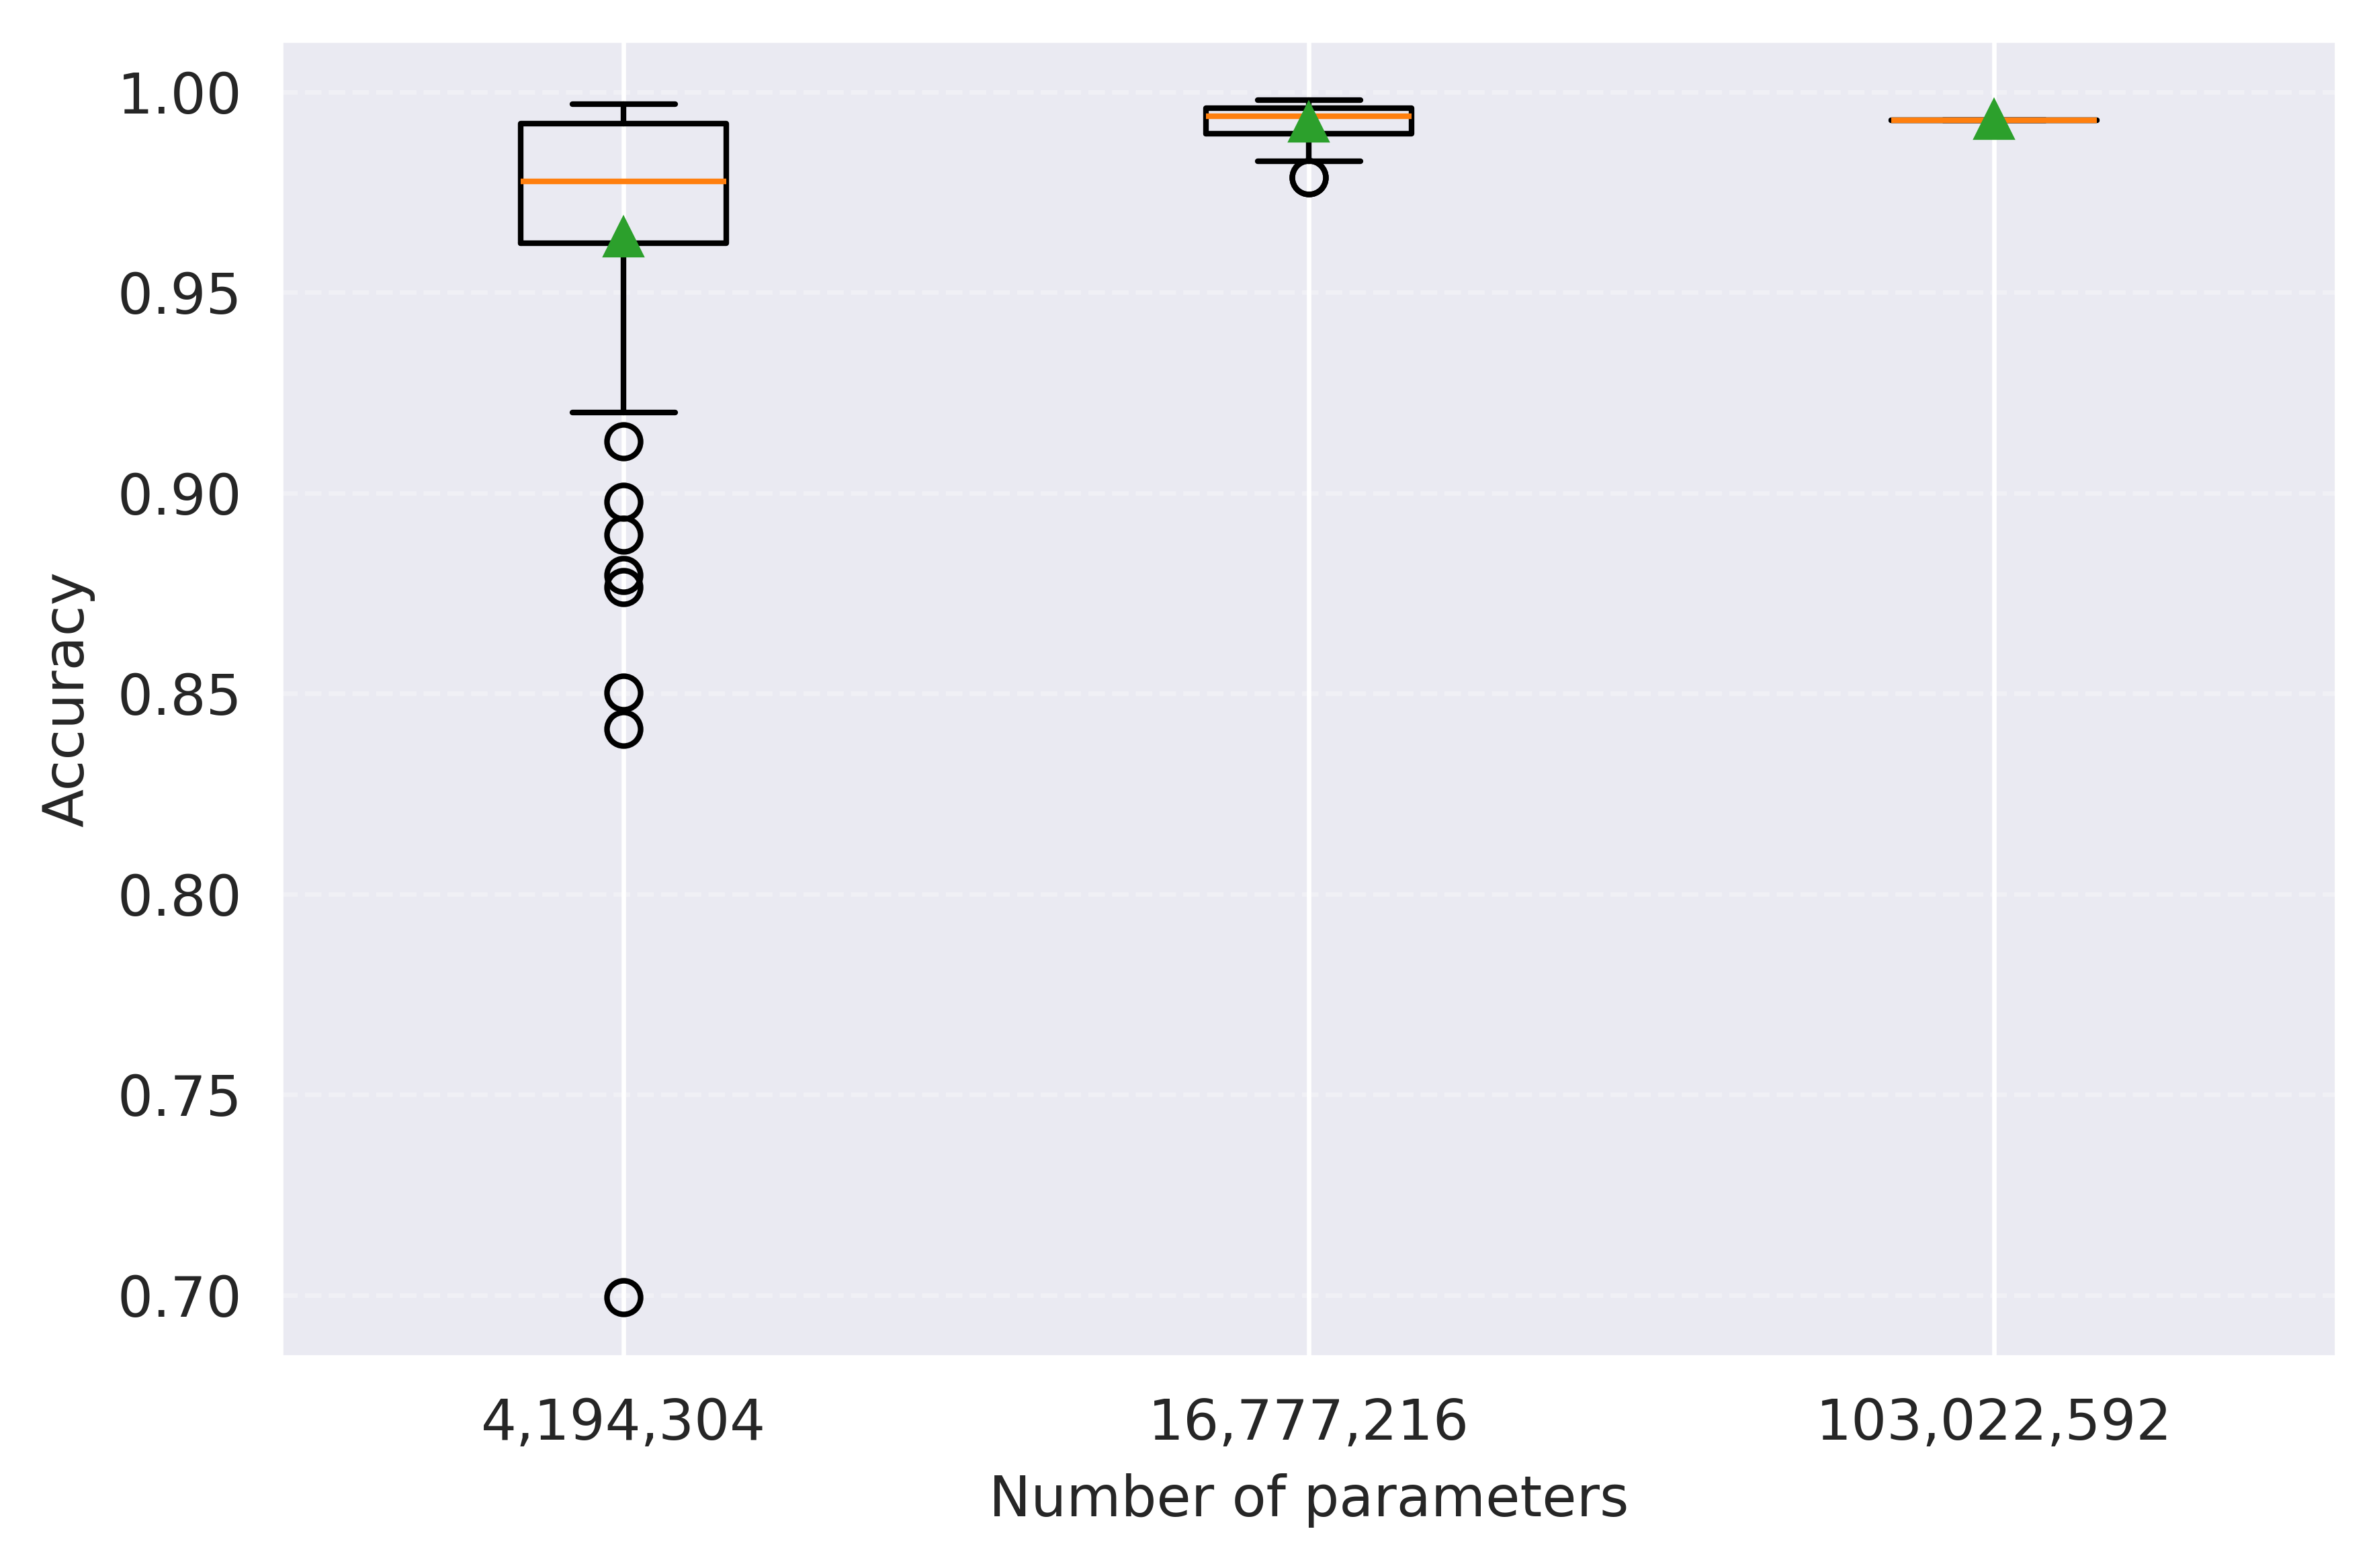
\includegraphics[width=\textwidth]{figures/results/paraphrased/accuracy_per_layer_boxplot.png}
        \caption{Paraphrased}
        \label{fig:accuracy_per_layer_boxplot_paraphrased}
    \end{subfigure}
    \hfill
    \begin{subfigure}[h]{0.495\textwidth}
        \centering
        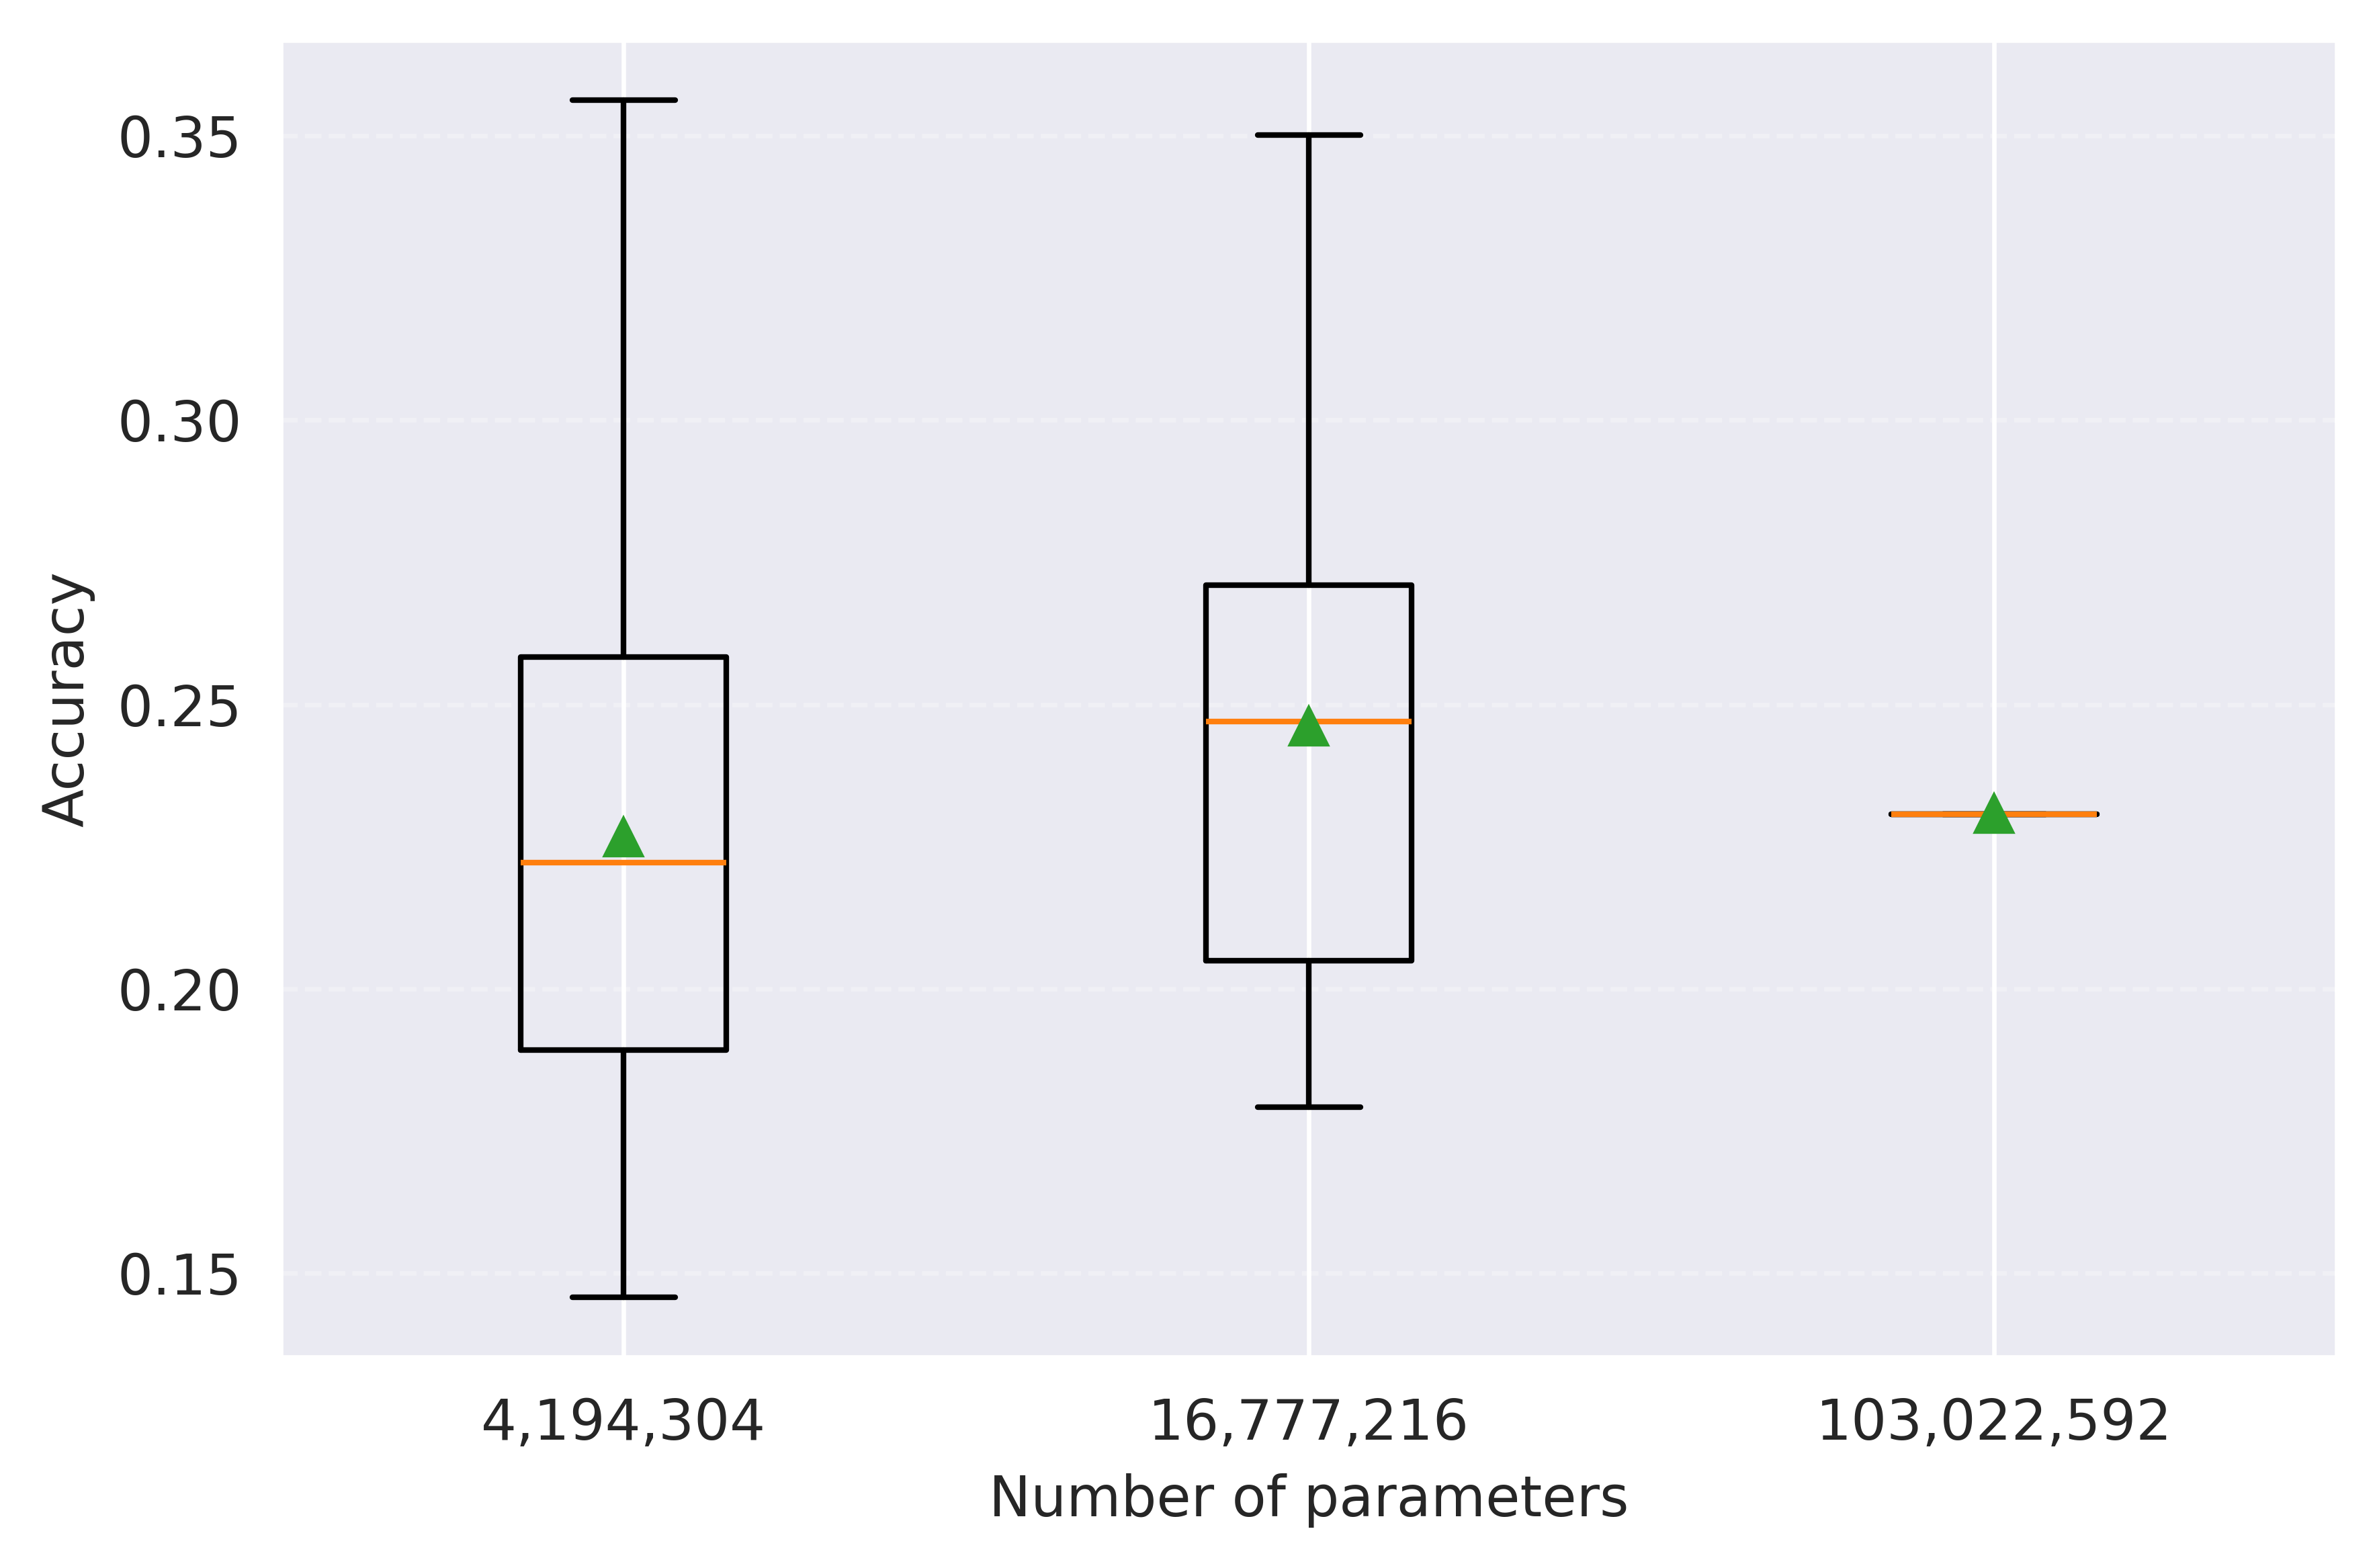
\includegraphics[width=\textwidth]{figures/results/model-generated/accuracy_per_layer_boxplot.png}
        \caption{Model-generated}
        \label{fig:accuracy_per_layer_boxplot_model_generated}
    \end{subfigure}
    \caption{Boxplots of of layer component accuracy with respect to the number of parameters}
    \label{fig:accuracy_per_layer_boxplot}
\end{figure}

\fxnote{add more text regarding accuracy}
\fxnote{how "well" does each layer find the most relevant sample to paraphrased samples}
\fxnote{maybe create plot with averages per layer type (k proj, q proj, etc.)}

\section{Comparison of Layer-Gradients and Full-Model-Gradient}\label{sec:layer_vs_full}
Faithfulness is quantified by computing the cosine similarity between the score vectors induced by $\vXspi[\W^{(l,k)}]$ and by $\vXspi[\theta]$. The dot-product formulation (Equations~\ref{eq:cosine_dot_full}–\ref{eq:cosine_dot_subset}) ensures these comparisons are reconstructed from the stored per-component dot products.
\begin{table}[h]
    \centering
    \begin{tabular}{|c|c|c|c|}
        \hline
        & \textbf{Layer Component} & \textbf{Paraphrased} & \textbf{Model-generated} \\
        \hline
        \multirow{1}{5em}{Embedding}
        & Embedding & 0.981 & 0.275 \\
        \hline
        \multirow{4}{5em}{Attention}
        & Query-Projection & 0.972 & 0.275 \\
        & Key-Projection & 0.9 & 0.201 \\
        & Value-Projection & 0.978 & 0.62 \\
        & Output-Projection & 0.988 & 0.63 \\
        \hline
        \multirow{3}{5em}{MLP}
        & Gate-Projection & 0.986 & 0.553 \\
        & Up-Projection & 0.988 & 0.571 \\
        & Down-Projection & 0.989 & 0.63 \\
        \hline
    \end{tabular}
    \caption{Average (median) cosine similarity between the scores of single layer components and the full gradient}
    \label{tab:average_cosine_similarity_full_gradient_comparison}
\end{table}

\fxnote{Which layers are most similar to the full-gradient, e.g. MLP, ATTN, Embeddings?}

\section{Greedy-Forward-Layer-Selection vs. Random Projections}\label{sec:greedy_vs_rp}
A forward greedy selection (Algorithm~\ref{alg:greedy_layer_selection}) is applied to build a subset of layer components whose \emph{combined} gradients best reproduce the full-model scores (objective $\rho$ in Equation~\ref{eq:rho_objective}). As a geometry-preserving baseline, a layer-wise random projection is used (Section~\ref{subsec:random_projection_as_a_baseline}) with target dimensions set to 1\% and 5\% of $M$. Both retrieval accuracy and cosine similarity to the full-model score vector are reported.

\subsection{Selection by Accuracy}
For each budget (number of selected components or projected dimension), $\operatorname{accuracy}^{(b)}$ is computed on $D_p$ and $D_m$ using $\mathcal{C}_i(b)$ with $b=5$.
\begin{figure}[h]
    \centering
    \begin{subfigure}[h]{0.49\textwidth}
        \centering
        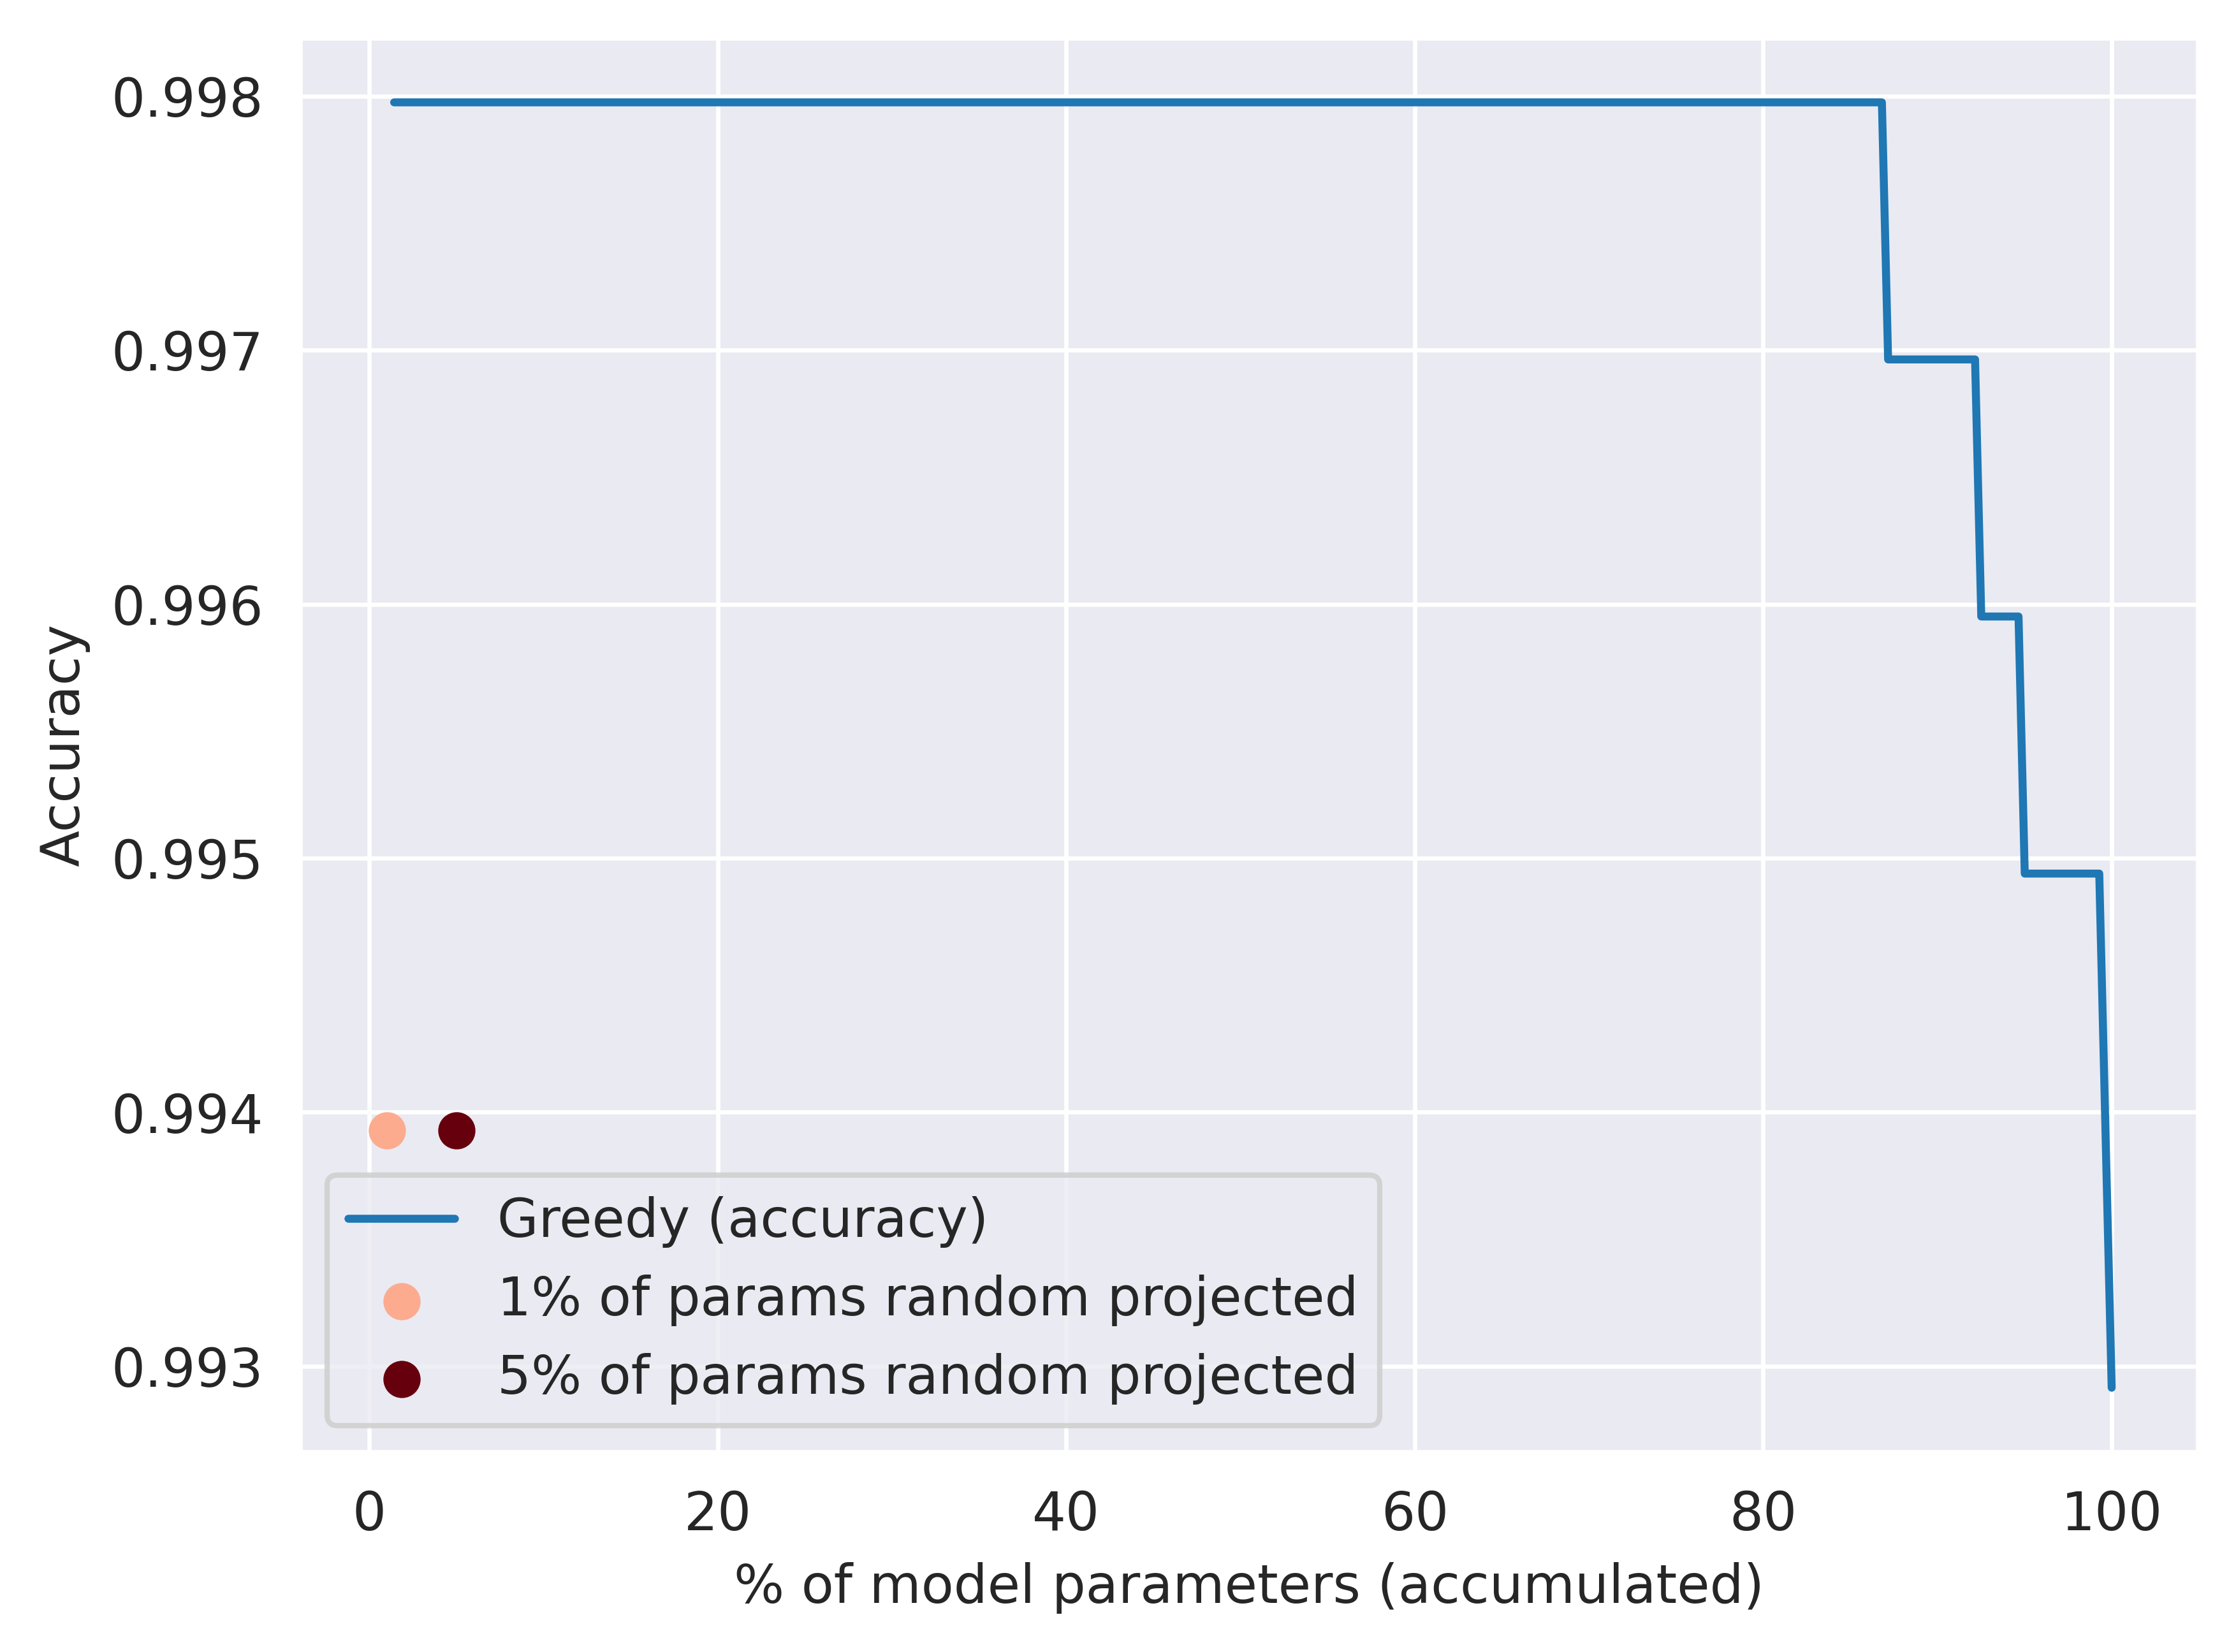
\includegraphics[width=\textwidth]{figures/results/paraphrased/greedy_layer_selection_accuracy.png}
        \caption{Paraphrased}
        \label{fig:greedy_layer_selection_accuracy_paraphrased}
    \end{subfigure}
    \hfill
    \begin{subfigure}[h]{0.49\textwidth}
        \centering
        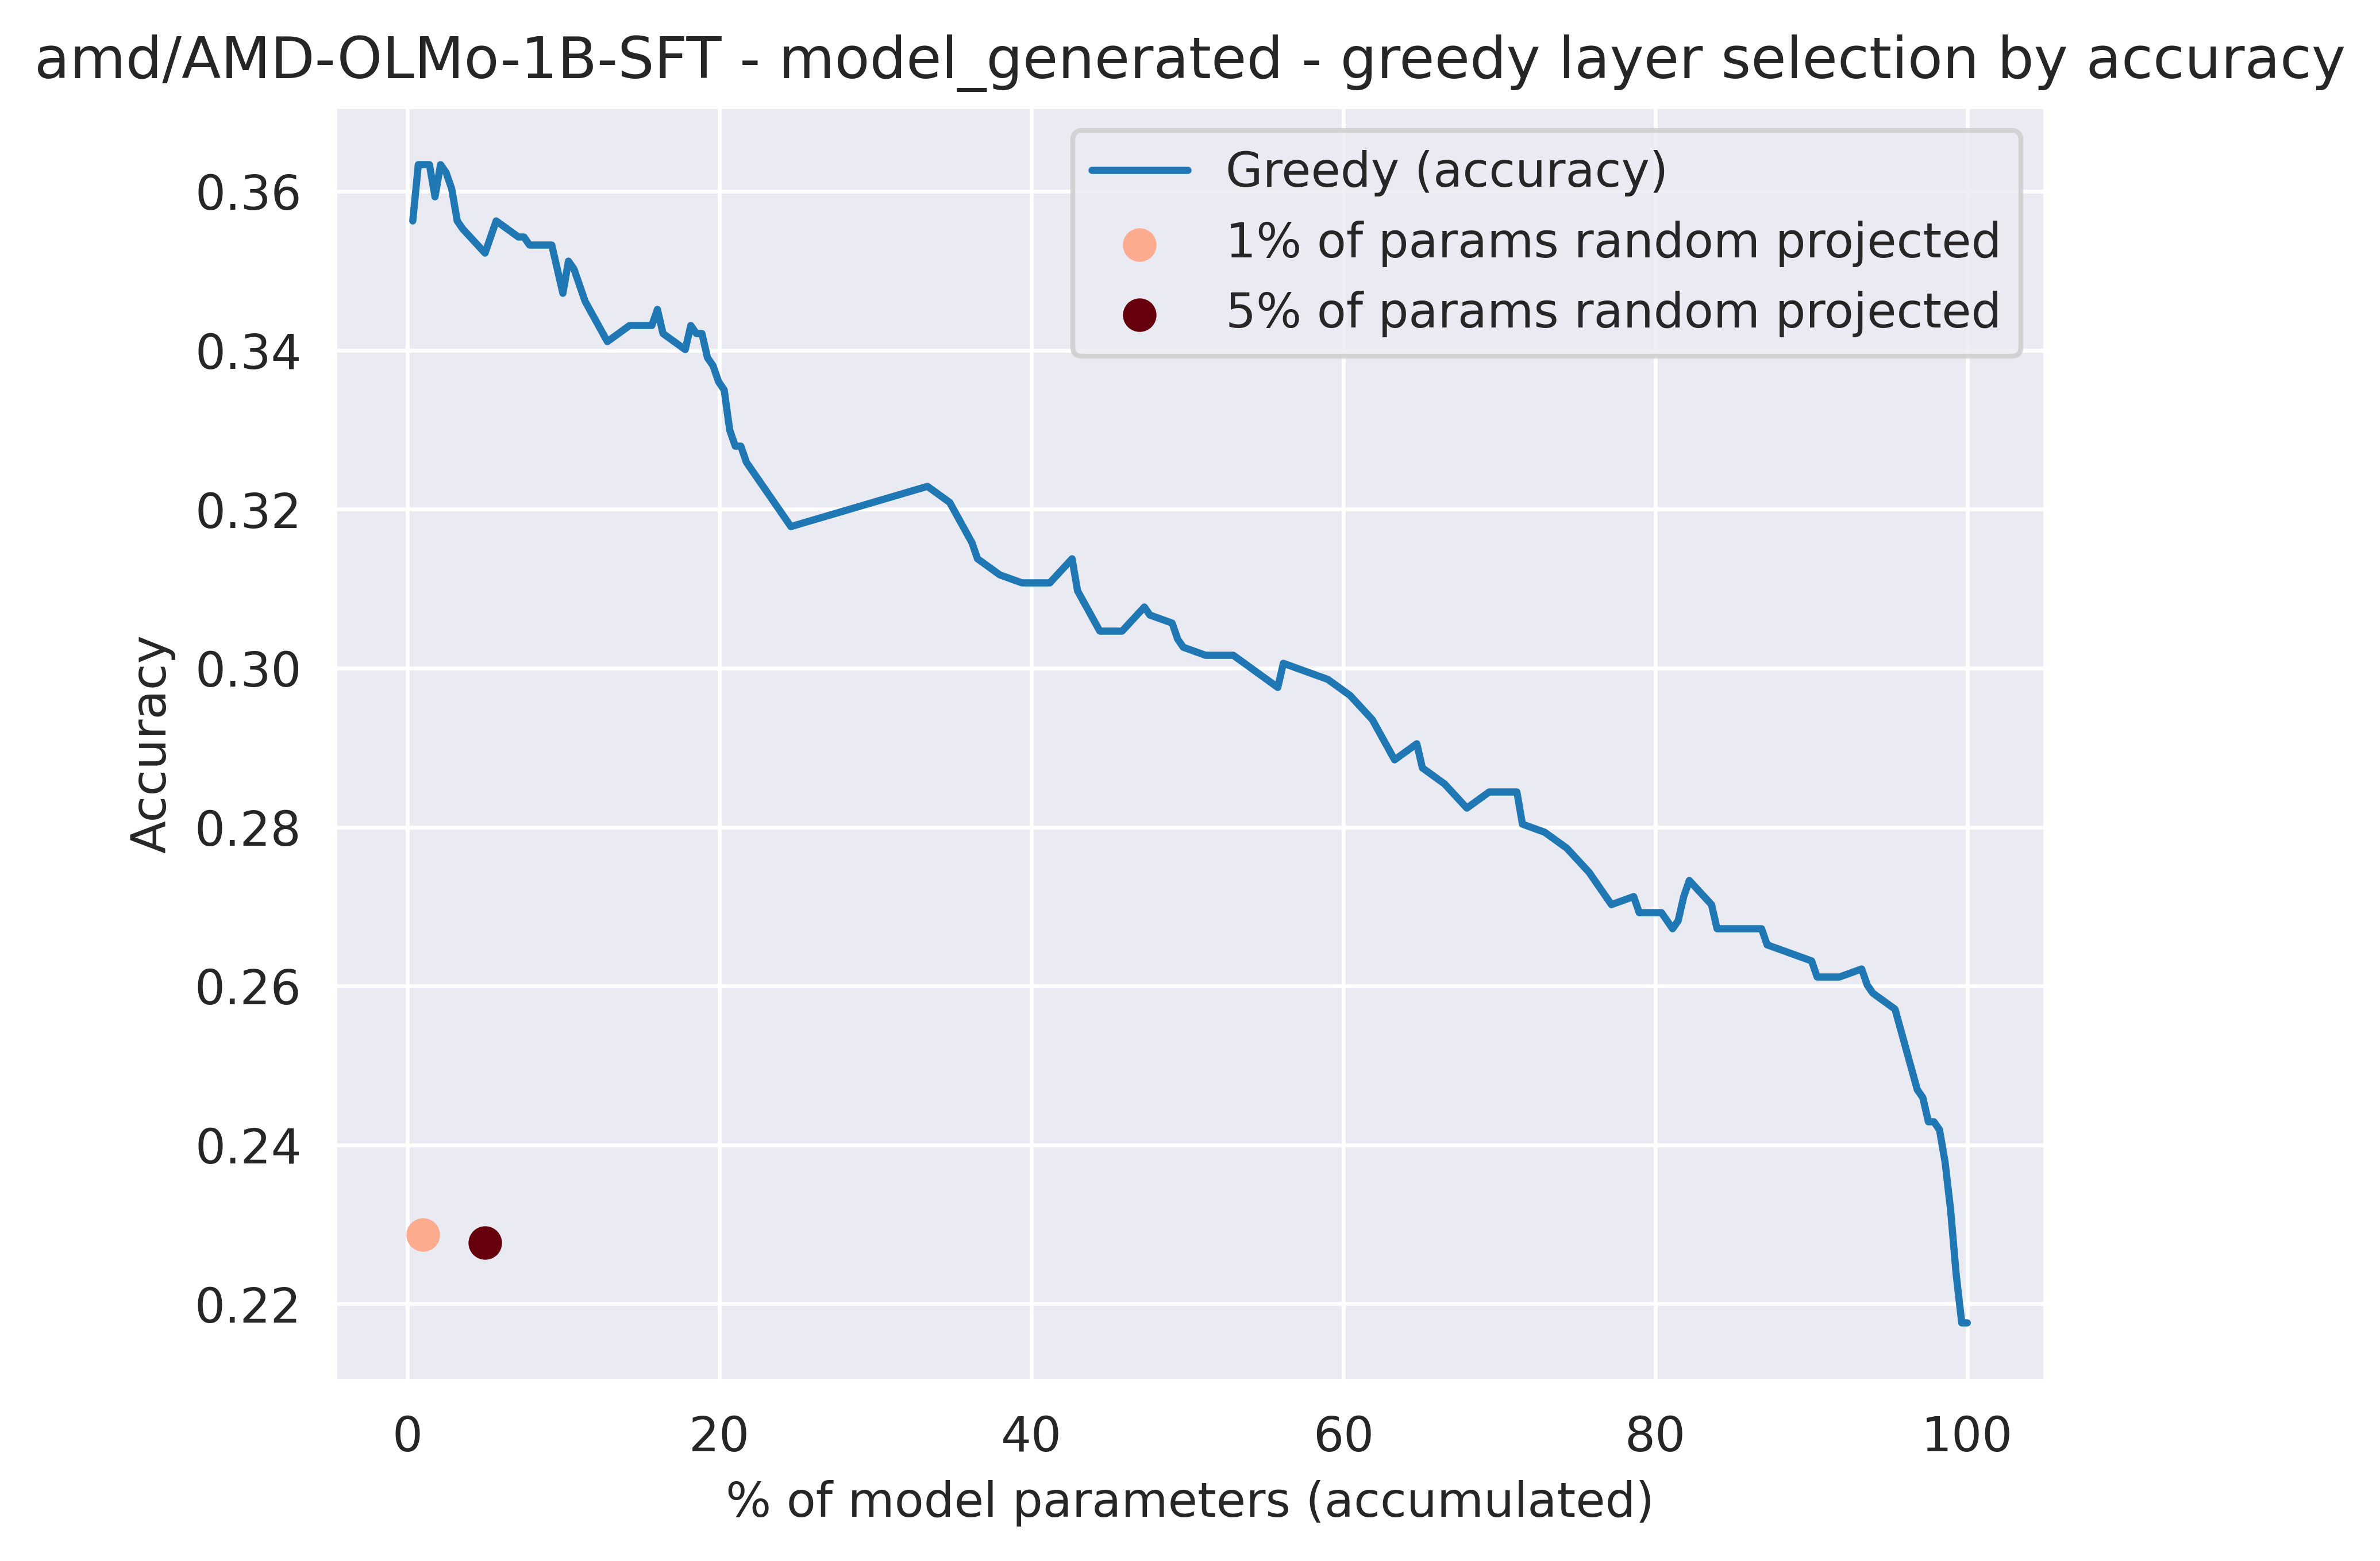
\includegraphics[width=\textwidth]{figures/results/model-generated/greedy_layer_selection_accuracy.png}
        \caption{Model-generated}
        \label{fig:greedy_layer_selection_accuracy_model_generated}
    \end{subfigure}
    \caption{Greedy Layer Selection and random projection by accuracy}
    \label{fig:greedy_layer_selection_accuracy}
\end{figure}

\subsection{Selection by Similarity to Full-Model-Gradient}
The objective $\rho(\mathcal{L})=\simcos(\hat{\Gamma}^{\mathcal{L}},\Gamma^\theta)$ (Equation~\ref{eq:rho_objective}) is tracked as components are added and compared to random projections of matched dimensionality.
\begin{figure}[h]
    \centering
    \begin{subfigure}[b]{0.49\textwidth}
        \centering
        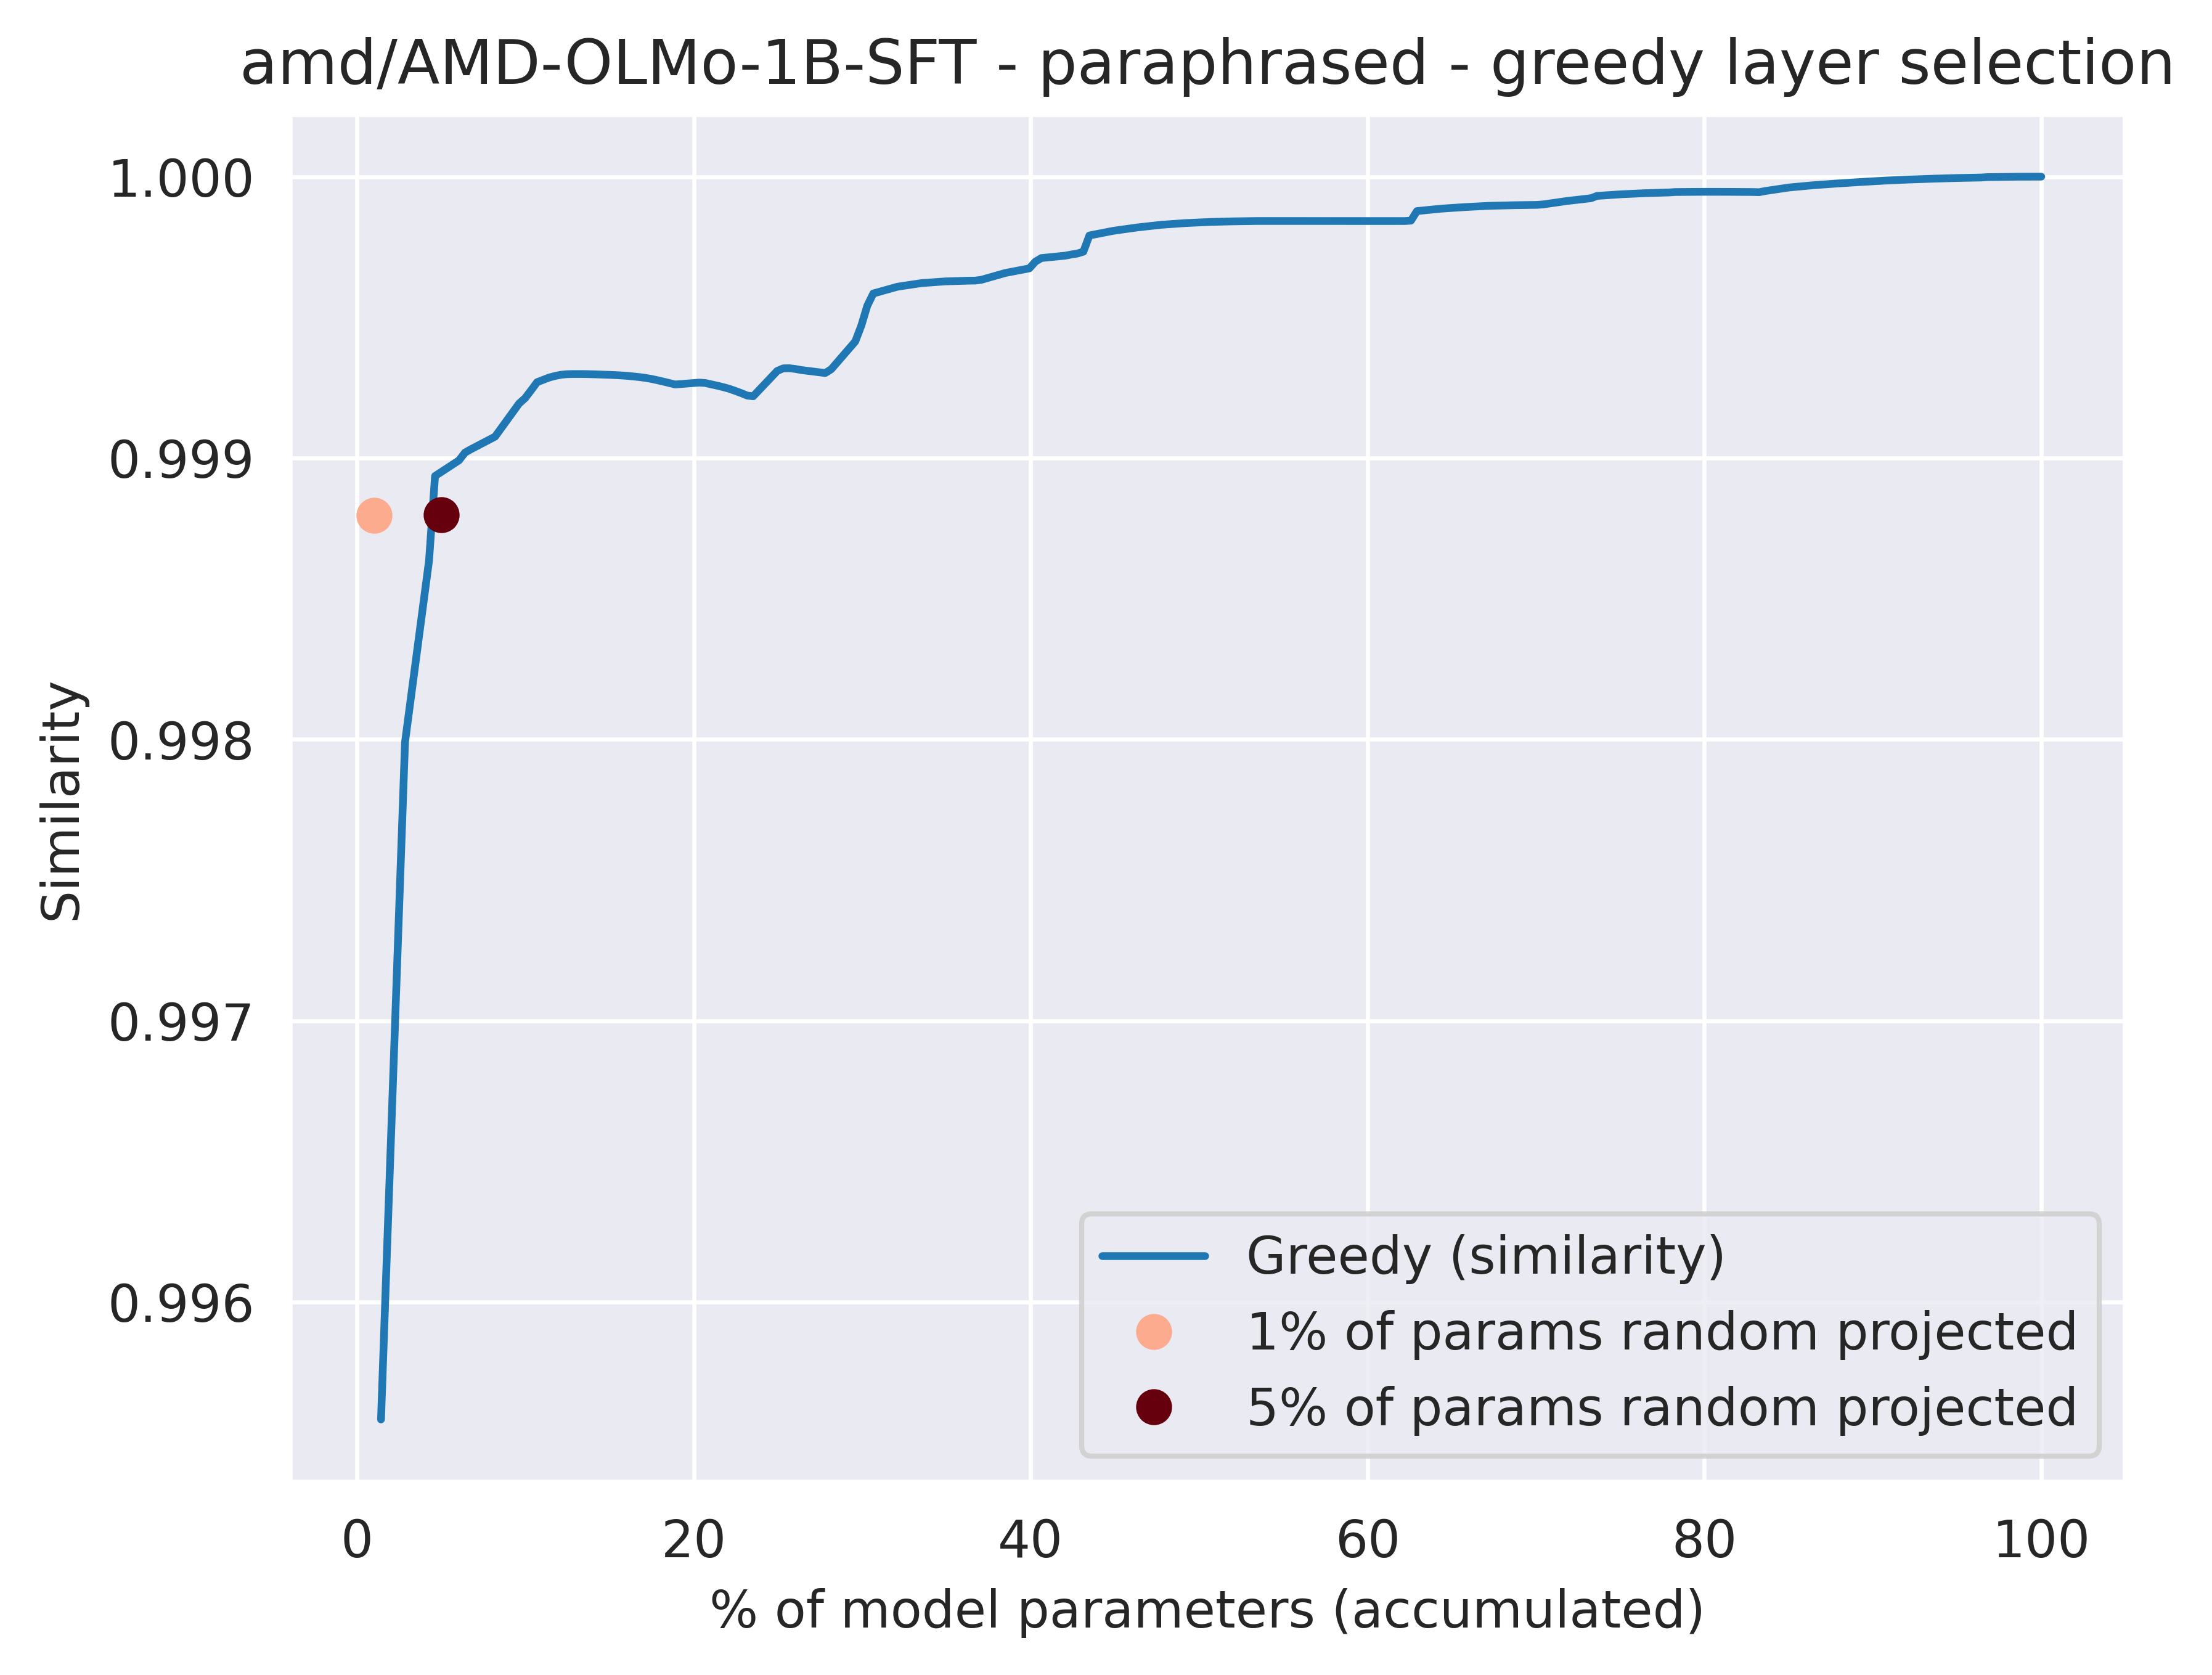
\includegraphics[width=\textwidth]{figures/results/paraphrased/greedy_layer_selection.png}
        \caption{Paraphrased}
        \label{fig:greedy_layer_selection_paraphrased}
    \end{subfigure}
    \hfill
    \begin{subfigure}[b]{0.49\textwidth}
        \centering
        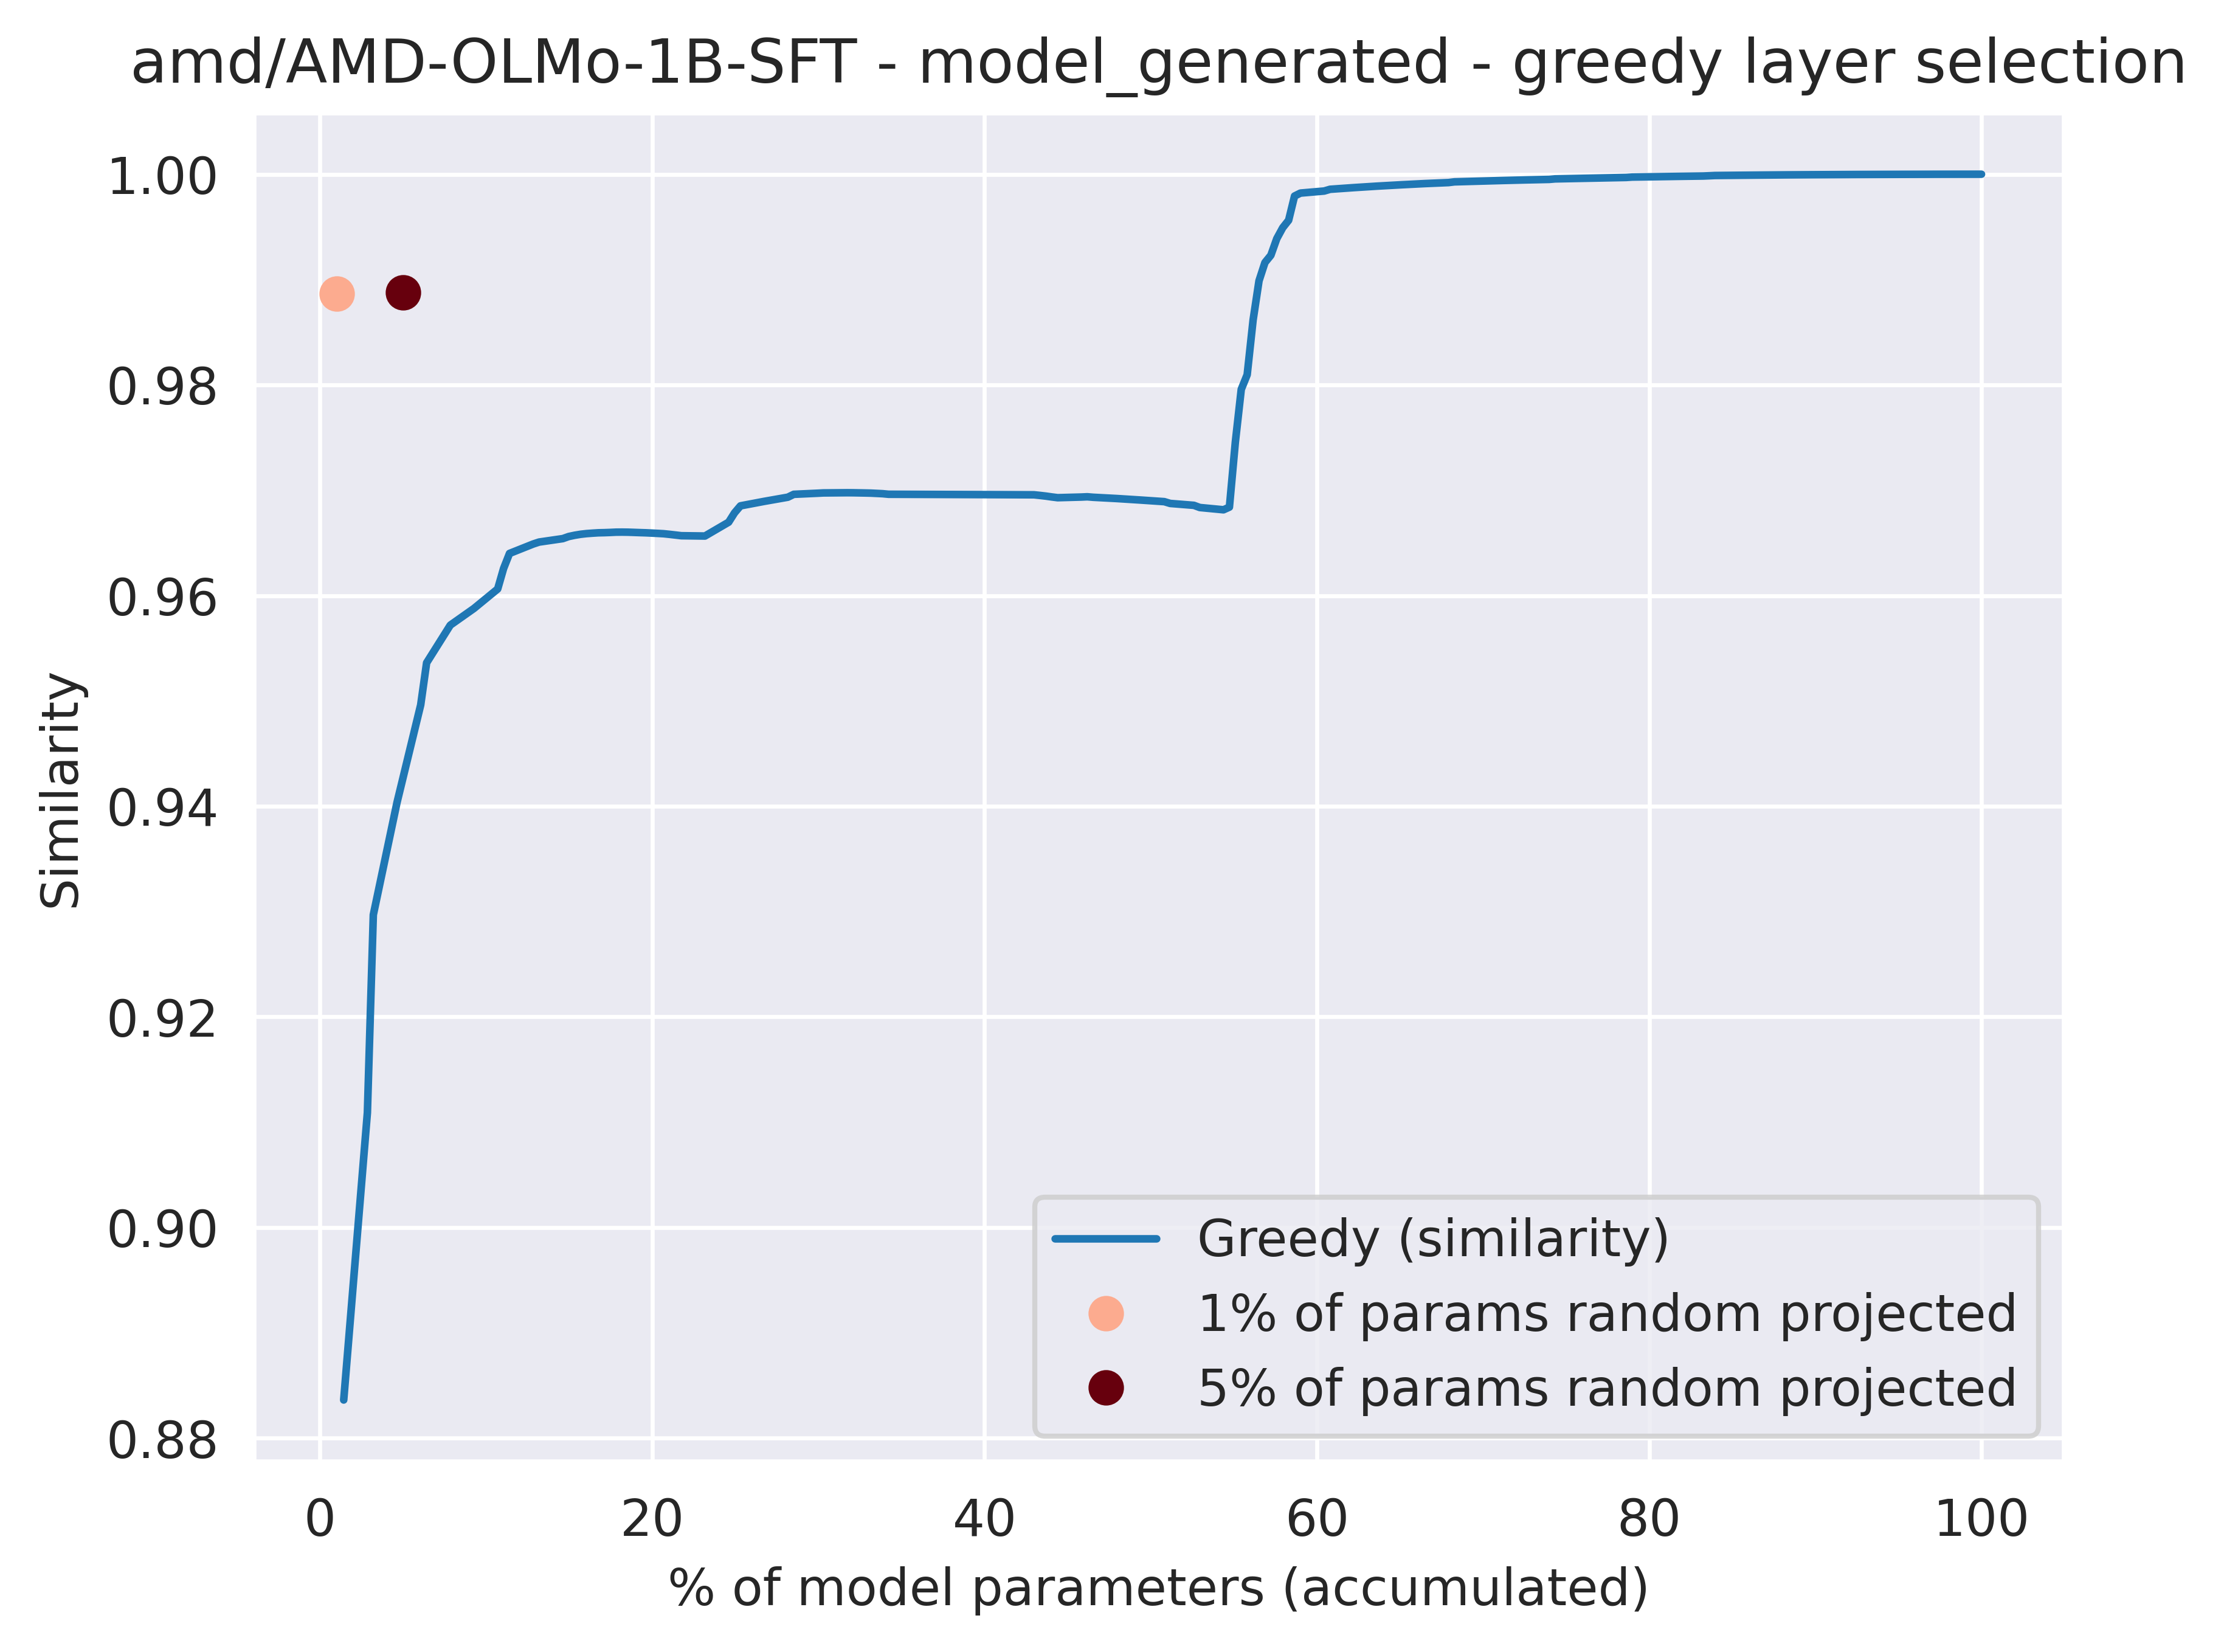
\includegraphics[width=\textwidth]{figures/results/model-generated/greedy_layer_selection.png}
        \caption{Model-generated}
        \label{fig:greedy_layer_selection_model_generated}
    \end{subfigure}
    \caption{Greedy Layer Selection compared to random projection by similarity to full model gradient}
    \label{fig:greedy_layer_selection}
\end{figure}

\section{Execution Time}\label{sec:exec_time}
Wall-clock times include dataset loading and all computations after model/tokenizer initialization. Each Slurm job logs its duration; totals are obtained by summing across jobs assigned to disjoint partitions. The report separates (i) computation of intermediate dot products (Section~\ref{subsec:intermediate_results}) and (ii) gradient-similarity evaluation with and without random projections.
\\\\
The execution time is measured after the model and the tokenizer is loaded. Hence, it contains the time to load the dataset from the disk and perform all computations. Each \emph{Slurm} job logs its execution time separately and saves it on disk for later inspections. To make the results comparable, the individual times from the jobs are summed. Table~\ref{tab:execution_times} shows the execution times on the hardware described above described in Section~\ref{sec:hardware}. In this context, \emph{dot-products} refers to the computation of the intermediate dot-products mentioned in Subsection~\ref{subsec:intermediate_results} and \emph{gradient similarity} refers to the calculation of cosine similarities for the gradients. 
\begin{table}[h]
    \centering
    \begin{tabular}{|l l|c|c|}
        \hline
        \textbf{Computation Type} & & \textbf{Paraphrased (h)} & \textbf{Model-generated (h)} \\
        \hline
        Dot-products & & 3.54 & 3.35 \\
        \hline
        \multirow{2}{*}{Gradient similarity} 
            & without RP & 4.05 & 5.39 \\
            & with RP & 927.48 & 925.63 \\
        \hline
    \end{tabular}
    \caption{Execution times (in hours) for dot-products and gradient similarity (with and without \acrfull{rp}) under paraphrased and model-generated settings.}
    \label{tab:execution_times}
\end{table}
